\section{Un exemple presque complet}\label{exemple}
%==========================================





	%%%%%%%%%%%%%%%%%%%%%%%%%%%%%%%%%%%%%%%%%%%%
	\begin{center}
	\footnotesize

	\definecolor{fastCouleurFondFS}{rgb}{0.90,0.85,0.70}
	\definecolor{fastCouleurFondFT}{rgb}{1,0.96,0.89}
	\definecolor{fastCouleurFondST}{rgb}{1,1,1}
	\renewcommand*{\fastHauteurBoite}{2.6em}
	\renewcommand*{\fastDecalageTrait}{-1.3em}
	\renewcommand*{\fastEspaceColonne}{9em}

	\begin{fast}{Déplacer la voiture téléguidée}
		\FT{Gérer les informations}
			{
			\FT{Démarrer la voiture}
				{
				\ST{Bouton marche/arrêt}
					[\FV{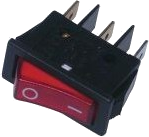
\includegraphics[height=1cm]{./sources_help/images/bouton.png}}]
				}
			\FT{Capter les ordres de la télécommande}
				{
				\ST{Antenne}
					[\FV{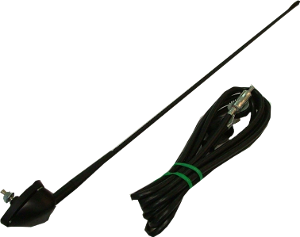
\includegraphics[height=1cm]{./sources_help/images/antenne.png}}]
				}
			\FT{Gérer les informations et distribuer}
				{
				\ST{Récepteur 2 voies}
					[\FV{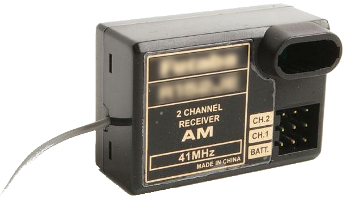
\includegraphics[height=1cm]{./sources_help/images/recepteur.png}}]
				}
			}
		\FT{Stocker l'énergie}
				{
				\trait{\ST{Batterie électrique}
					[\FV{
\includegraphics[height=1cm]{./sources_help/images/batterie.png}}]
				}}
		\FT{Propulser la voiture}
			{
			\FT{Transformer en énergie mécanique}
				{
				\ST{Moteur à courant continu}
					[\FV{
\includegraphics[height=1cm]{./sources_help/images/moteur.png}}]
				}
			\FT{Adapter l'énergie mécanique}
				{
				\ST{Engrenages}
					[\FV{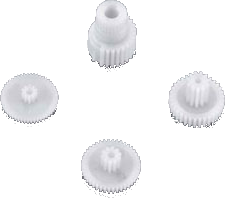
\includegraphics[height=1cm]{./sources_help/images/pignons.png}}]
				}
			\FT{Transmettre l'énergie mécanique}
				{
				\ST{Roues}
					[\FV{
\includegraphics[height=1cm]{./sources_help/images/roue.png}}]
				}
			}
		\FT{Diriger la voiture}
			{
			\FT{Transformer l'énergie}
				{
				\ST{Servomoteur}
					[\FV{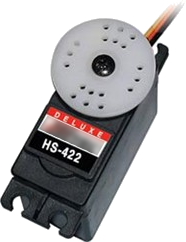
\includegraphics[height=1cm]{./sources_help/images/servomoteur.png}}]
				}
			\FT{Transmettre aux roues}
				{
				\ST{Biellettes}
					[\FV{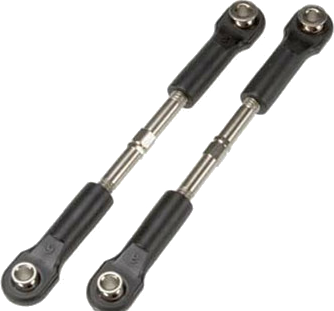
\includegraphics[height=1cm]{./sources_help/images/biellettes.png}}]
				}
			}
	\end{fast}
	\fastReset
	\end{center}
	%%%%%%%%%%%%%%%%%%%%%%%%%%%%%%%%%%%%%%%%%%%%


	L'exemple ci-dessus est donné par le code suivant :

%######################################
\begin{lstlisting}
\begin{center}
\footnotesize

\definecolor{fastCouleurFondFS}{rgb}{0.90,0.85,0.70}
\definecolor{fastCouleurFondFT}{rgb}{1,0.96,0.89}
\definecolor{fastCouleurFondST}{rgb}{1,1,1}
\renewcommand*{\fastHauteurBoite}{2.6em}
\renewcommand*{\fastDecalageTrait}{-1.3em}
\renewcommand*{\fastEspaceColonne}{9em}

\begin{fast}{Déplacer la voiture téléguidée}
	\FT{Gérer les informations}
		{\FT{Démarrer la voiture}
			{\ST{Bouton marche/arrêt}
				[\FV{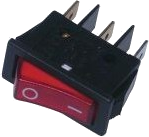
\includegraphics[height=1cm]
				{./sources_help/images/bouton.png}}]
			}
		\FT{Capter les ordres de la télécommande}
			{\ST{Antenne}
				[\FV{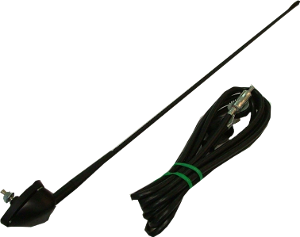
\includegraphics[height=1cm]
				{./sources_help/images/antenne.png}}]
			}
		\FT{Gérer les informations et distribuer}
			{\ST{Récepteur 2 voies}
				[\FV{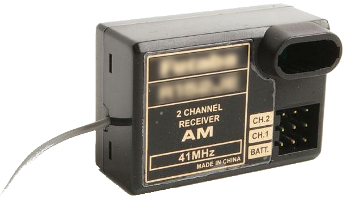
\includegraphics[height=1cm]
				{./sources_help/images/recepteur.png}}]
		}	}
	\FT{Stocker énergie}
		{\trait{
			\ST{Batterie électrique}
				[\FV{
\includegraphics[height=1cm]
				{./sources_help/images/batterie.png}}]
		}	}
	\FT{Propulser la voiture}
		{\FT{Transformer en énergie mécanique}
			{\ST{Moteur à courant continu}
				[\FV{
\includegraphics[height=1cm]
				{./sources_help/images/moteur.png}}]
			}
		\FT{Adapter l'énergie mécanique}
			{\ST{Engrenages}
				[\FV{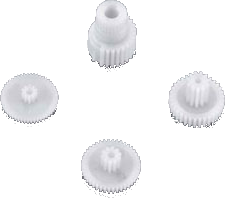
\includegraphics[height=1cm]
				{./sources_help/images/pignons.png}}]
			}
		\FT{Transmettre l'énergie mécanique}
			{\ST{Roues}
				[\FV{
\includegraphics[height=1cm]
				{./sources_help/images/roue.png}}]
		}	}
	\FT{Diriger la voiture}
		{\FT{Transformer l'énergie}
			{\ST{Servomoteur}
				[\FV{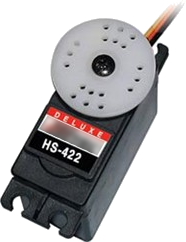
\includegraphics[height=1cm]
				{./sources_help/images/servomoteur.png}}]
			}
		\FT{Transmettre aux roues}
			{\ST{Biellettes}
				[\FV{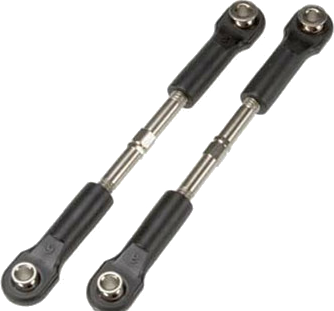
\includegraphics[height=1cm]
				{./sources_help/images/biellettes.png}}]
		}	}
\end{fast}
\fastReset
\end{center}
\end{lstlisting}
	
